\section{Appendix B: Supplementary Forecasting Results}

This appendix gathers the extra forecasting diagnostics and model-comparison plots that complement the main discussion. It leans on figures rather than tables: changes in model behaviour come through far more clearly in a picture than in a very wide table.

\subsection{Model-comparison figures}

\begin{figure}[H]
    \centering
    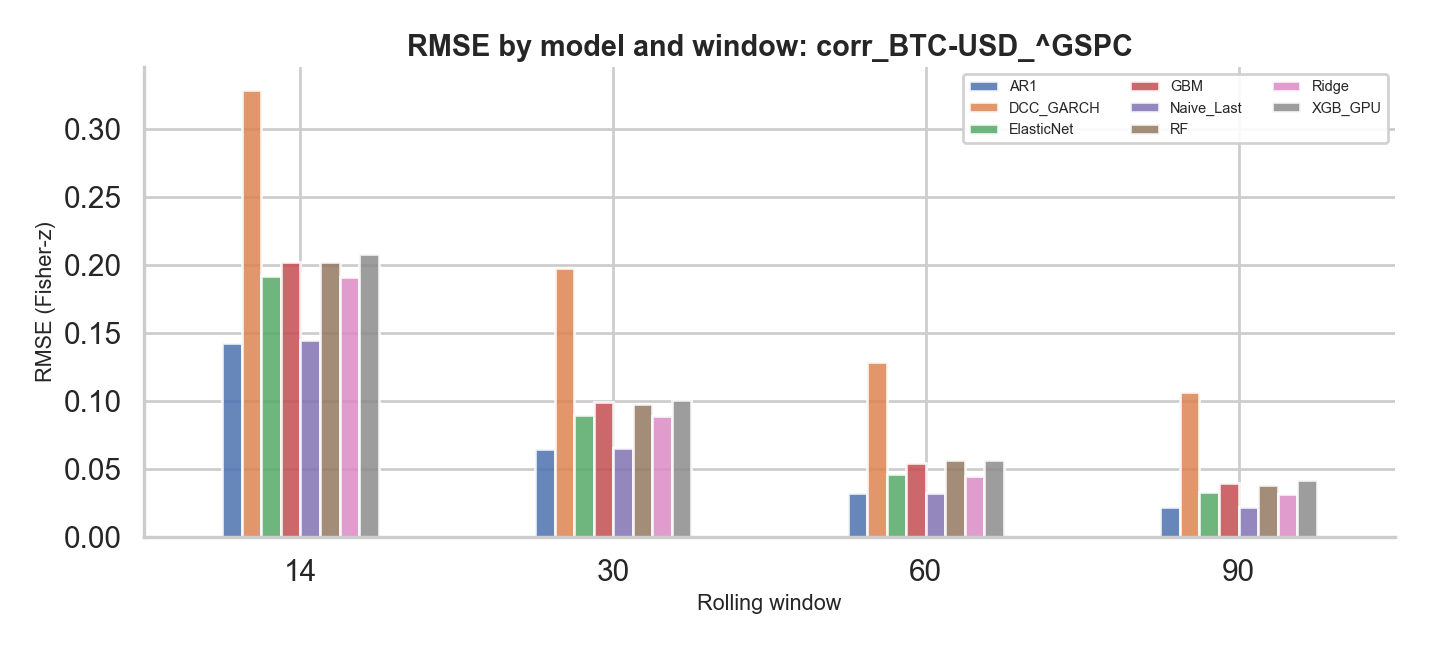
\includegraphics[width=0.8\textwidth]{../outputs/figures/model_rmse_comparison.png}
    \caption{Average RMSE comparison across model families.}
    \label{fig:app_rmse_comparison}
\end{figure}

\begin{figure}[H]
    \centering
    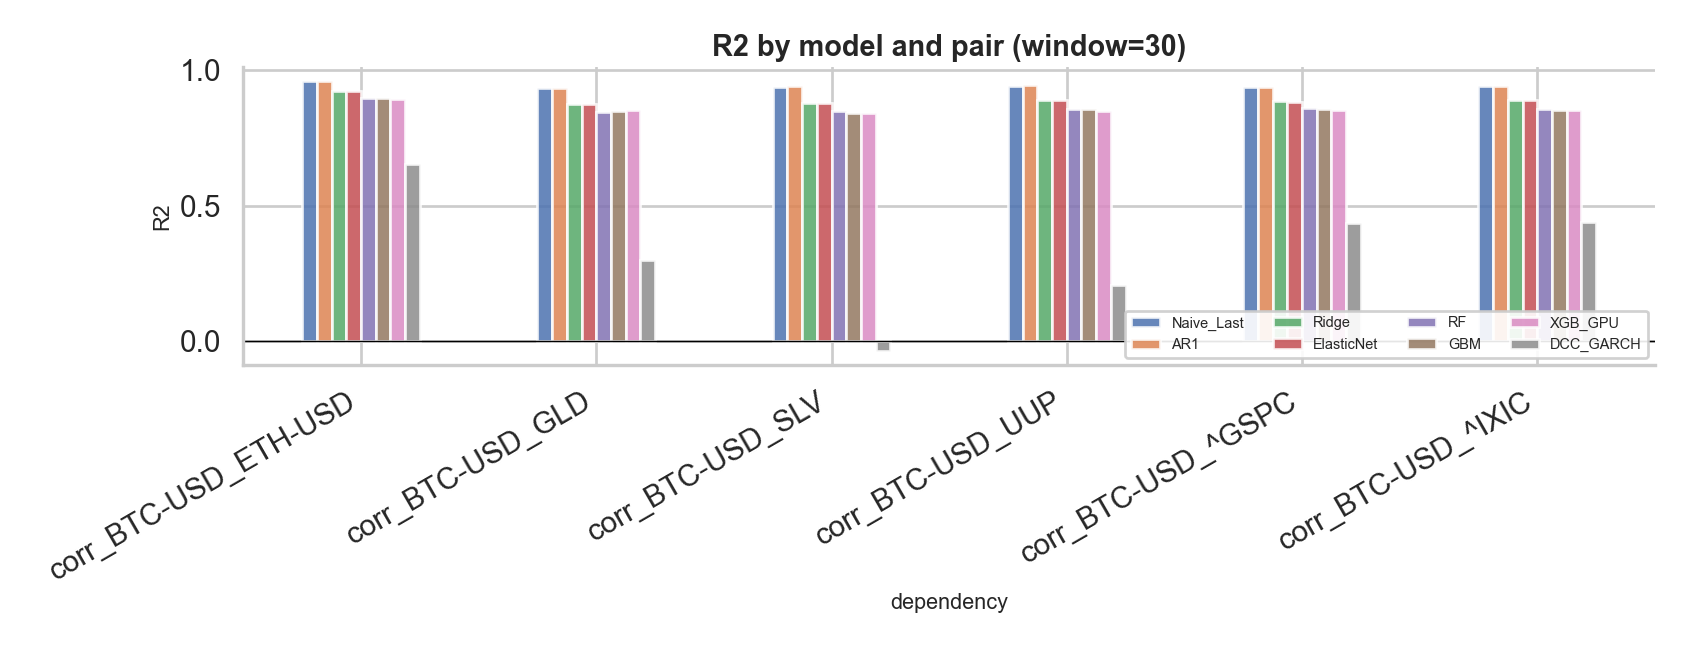
\includegraphics[width=0.8\textwidth]{../outputs/figures/model_r2_comparison_w30.png}
    \caption{Model $R^2$ comparison for the 30-day window.}
    \label{fig:app_r2_comparison}
\end{figure}

\begin{figure}[H]
    \centering
    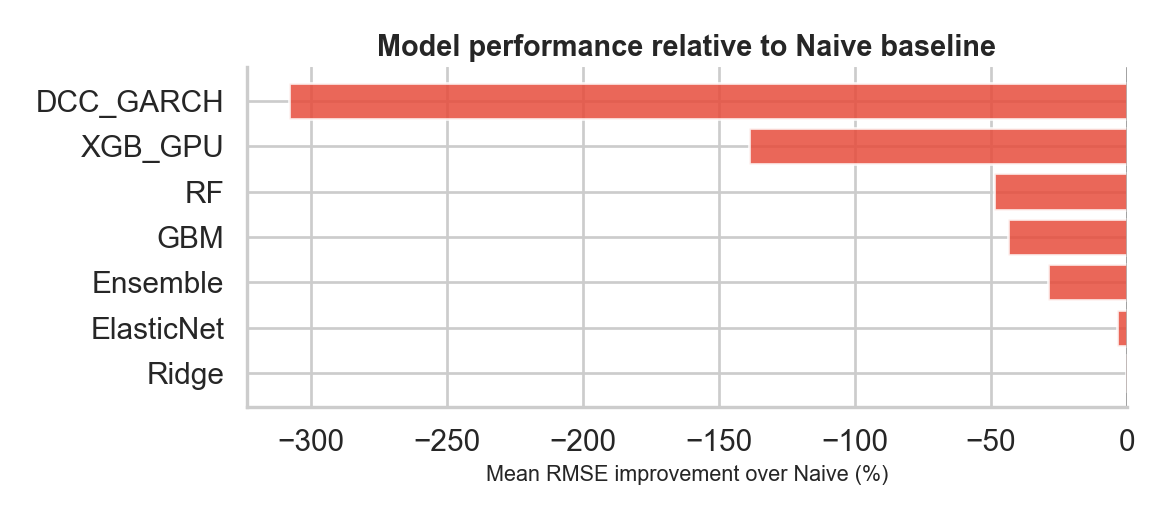
\includegraphics[width=0.8\textwidth]{../outputs/figures/model_improvement_over_naive.png}
    \caption{Improvement relative to the naive baseline.}
    \label{fig:app_improvement_naive}
\end{figure}

\subsection{Hyperparameter and feature diagnostics}

\begin{figure}[H]
    \centering
    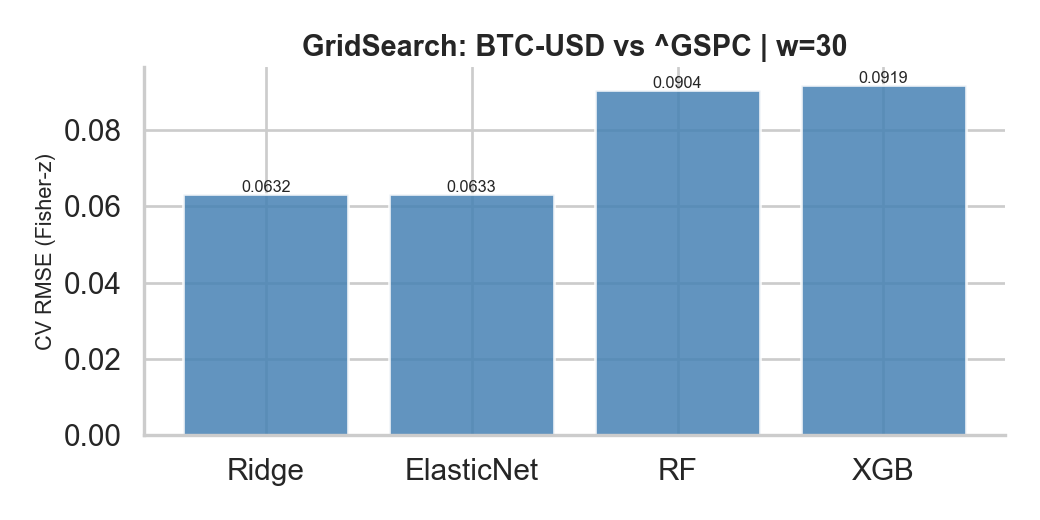
\includegraphics[width=0.8\textwidth]{../outputs/figures/gridsearch_cv_rmse_BTC-USD_^GSPC_w30.png}
    \caption{Grid-search cross-validation RMSE for the representative Bitcoin--S\&P 500 forecasting task.}
    \label{fig:app_gridsearch}
\end{figure}

\begin{figure}[H]
    \centering
    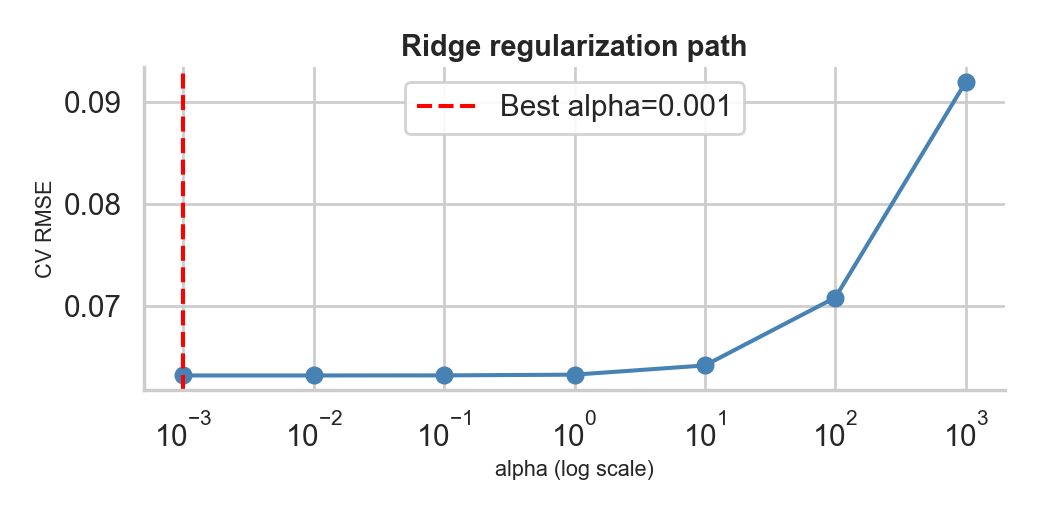
\includegraphics[width=0.8\textwidth]{../outputs/figures/ridge_regularization_path.png}
    \caption{Regularization path for the Ridge-based forecasting specification.}
    \label{fig:app_ridge_path}
\end{figure}

\begin{figure}[H]
    \centering
    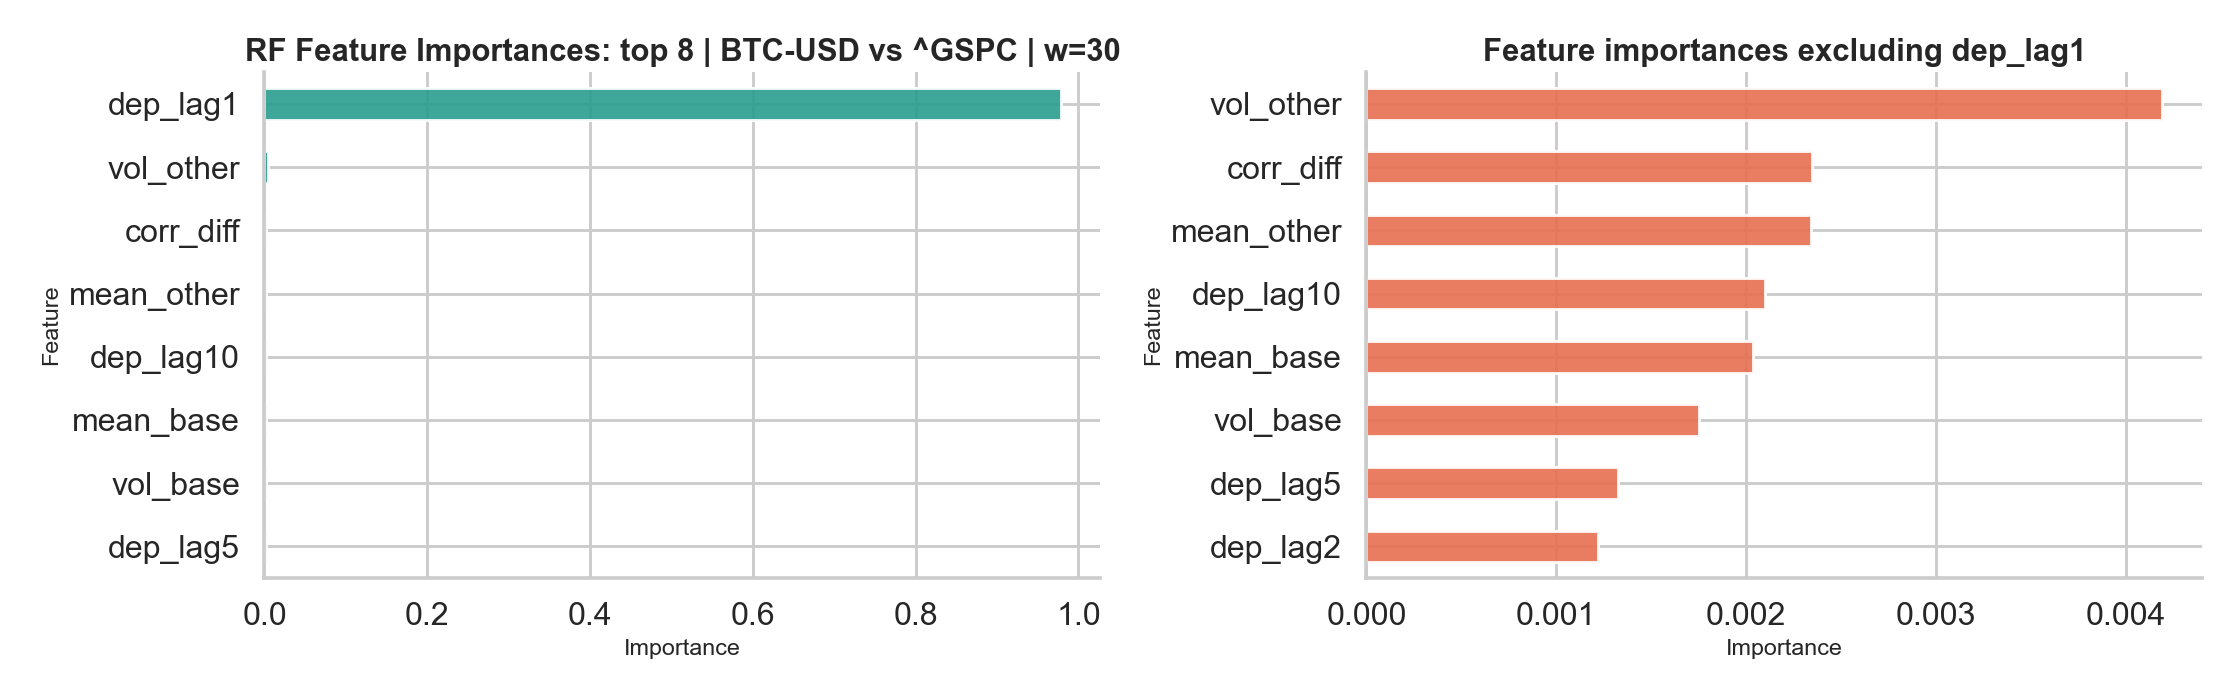
\includegraphics[width=0.85\textwidth]{../outputs/figures/rf_feature_importance_BTC-USD_^GSPC_w30_readable.png}
    \caption{Readable feature-importance view for the Random Forest model.}
    \label{fig:app_rf_importance}
\end{figure}

\subsection{Diagnostic plots for the representative equity pair}

\begin{figure}[H]
    \centering
    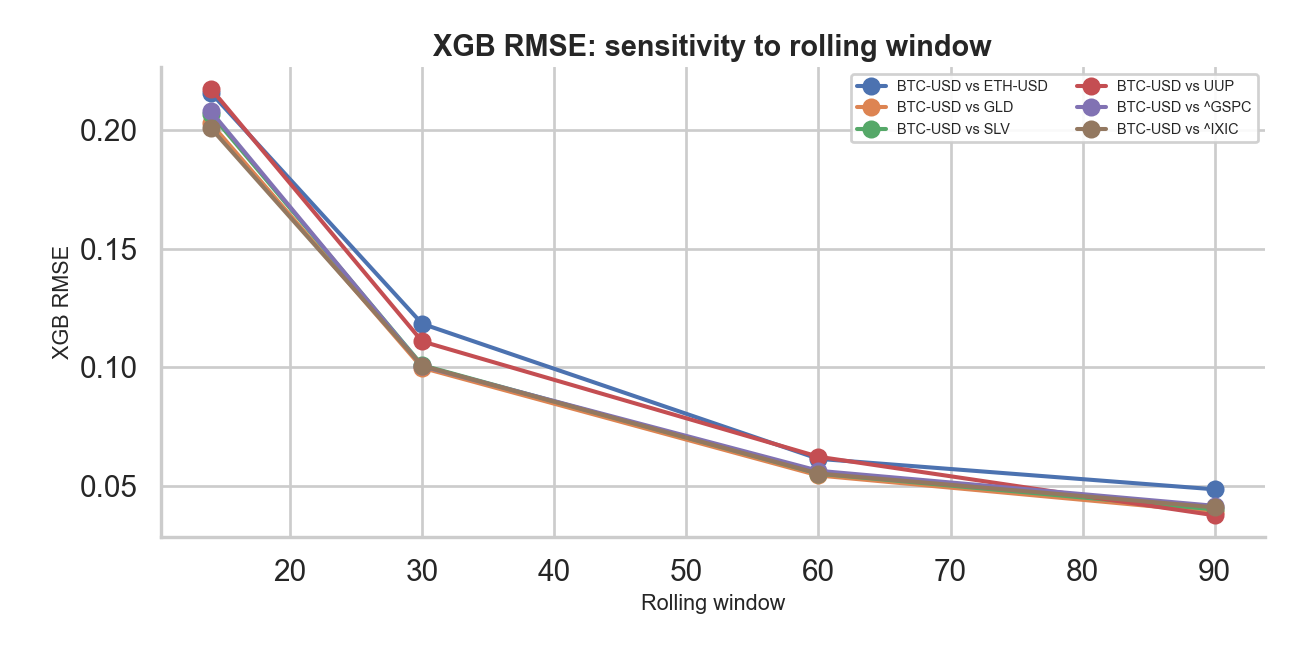
\includegraphics[width=0.82\textwidth]{../outputs/figures/xgb_window_sensitivity.png}
    \caption{Window sensitivity of the XGBoost-based forecasting layer.}
    \label{fig:app_xgb_sensitivity}
\end{figure}

\begin{figure}[H]
    \centering
    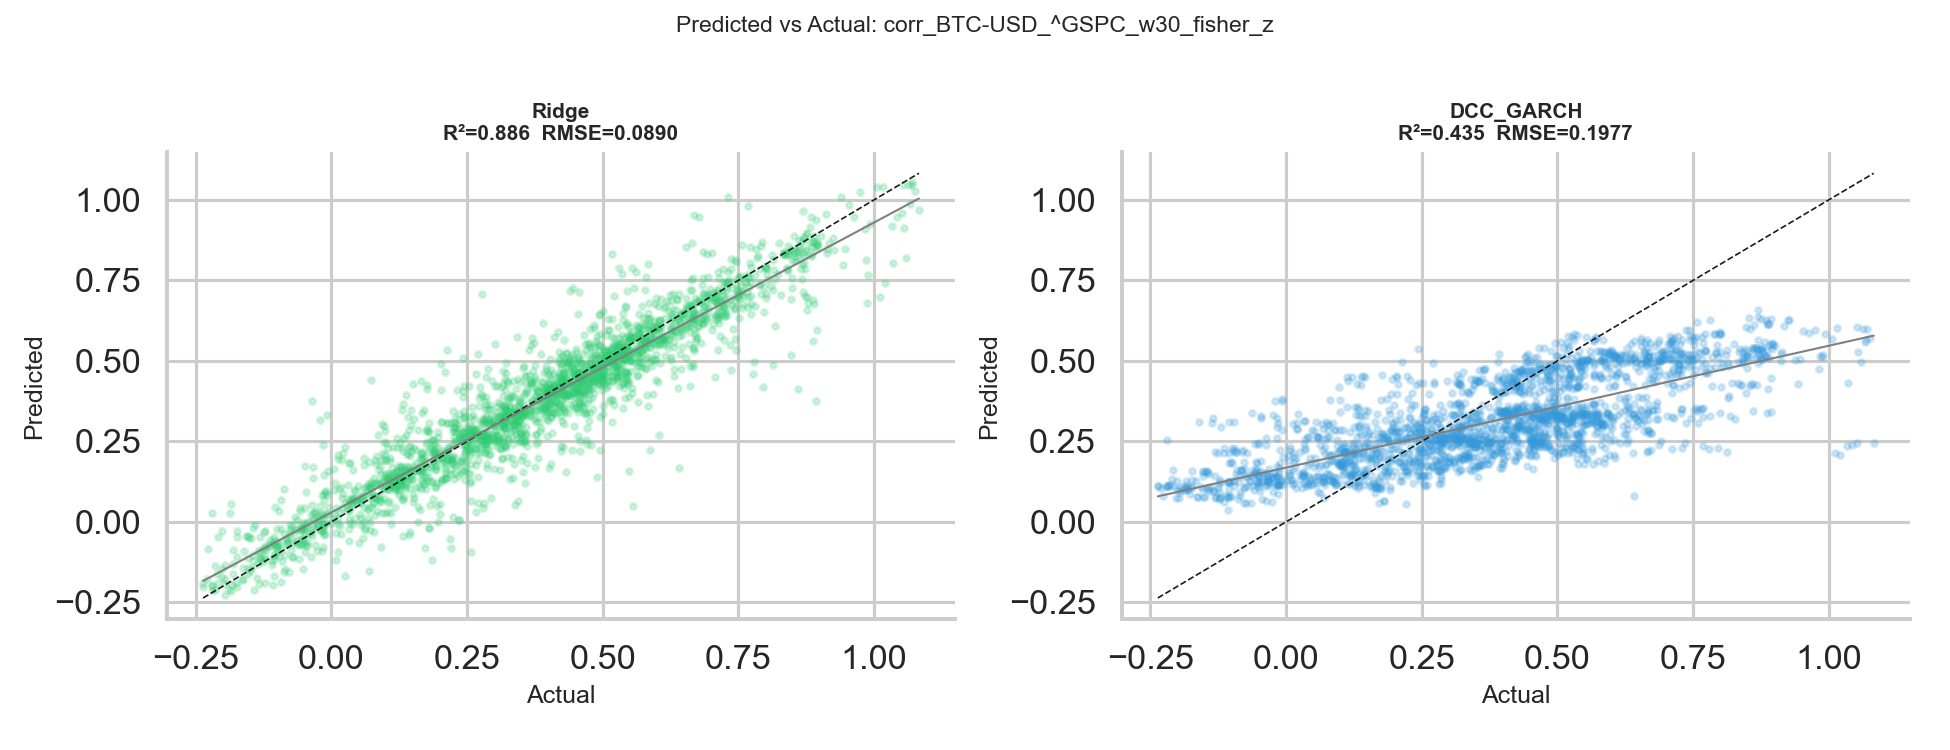
\includegraphics[width=0.82\textwidth]{../outputs/figures/scatter_corr_BTC-USD_^GSPC_w30_fisher_z.png}
    \caption{Forecast scatter diagnostic for the Bitcoin--S\&P 500 dependency experiment.}
    \label{fig:app_scatter_gspc}
\end{figure}

\begin{figure}[H]
    \centering
    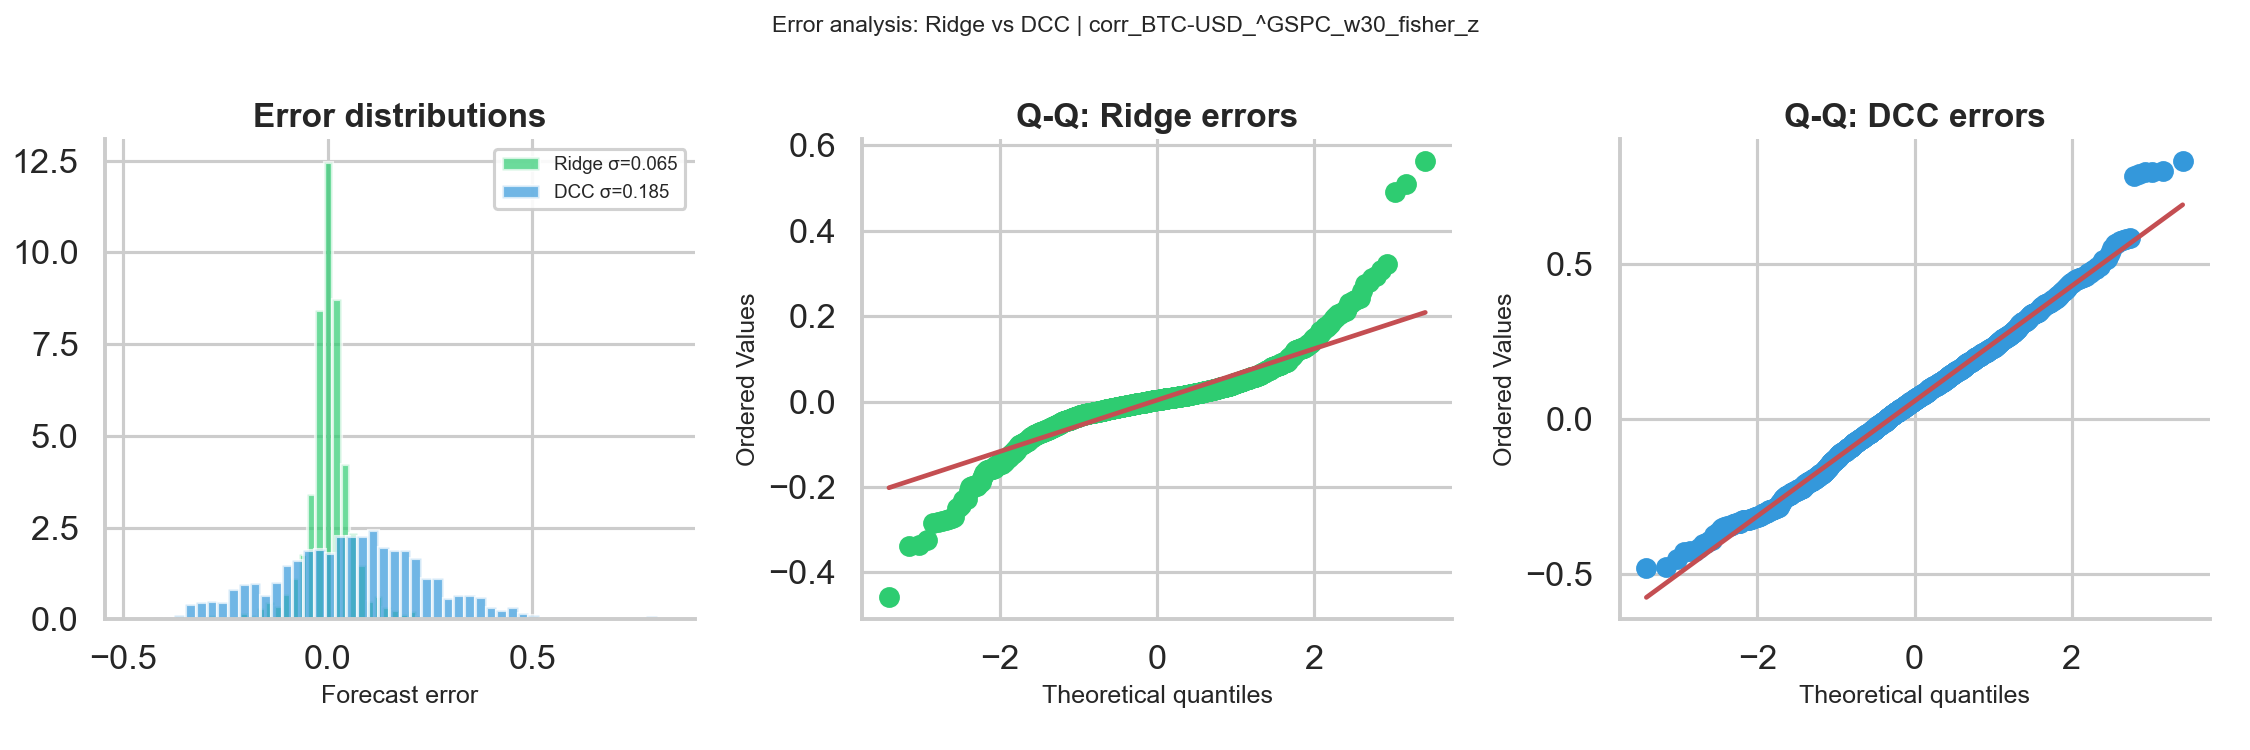
\includegraphics[width=0.82\textwidth]{../outputs/figures/error_dist_corr_BTC-USD_^GSPC_w30_fisher_z.png}
    \caption{Forecast error distribution for the representative Bitcoin--S\&P 500 dependency experiment.}
    \label{fig:app_error_dist_gspc}
\end{figure}

\subsection{Sensitivity by asset pair}

\begin{figure}[H]
    \centering
    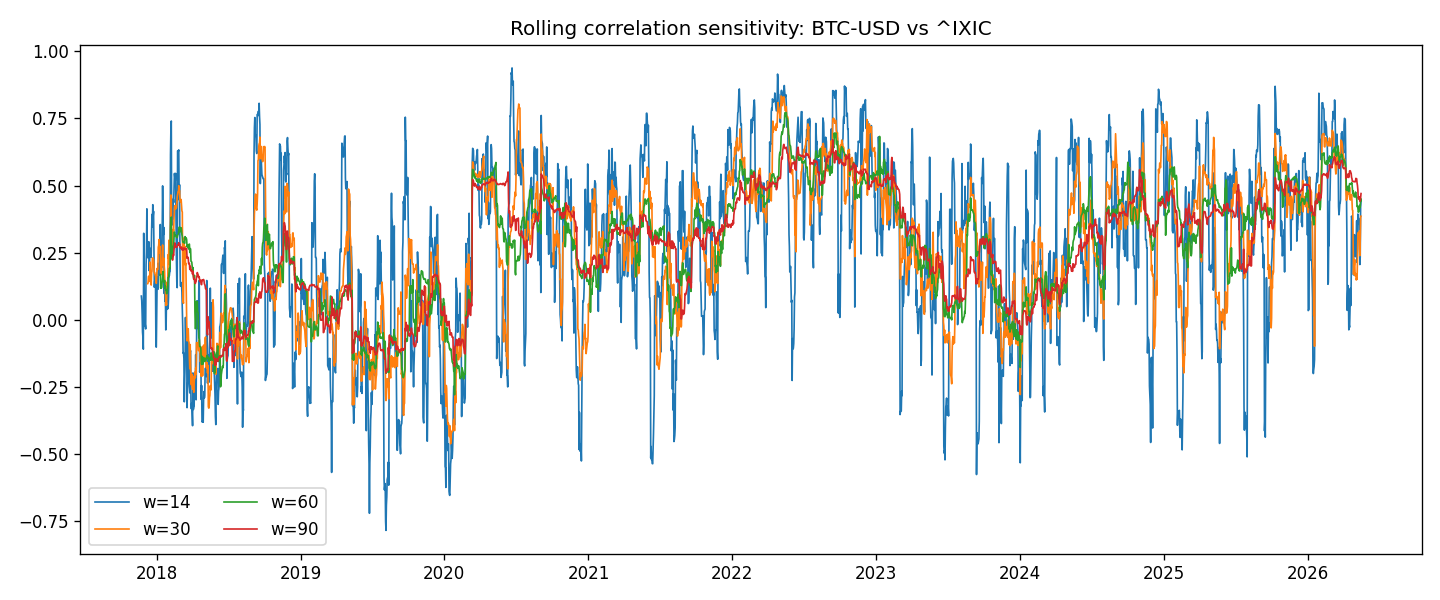
\includegraphics[width=0.9\textwidth]{../outputs/figures/sensitivity_BTC-USD_^IXIC.png}
    \caption{Sensitivity analysis for the Bitcoin--NASDAQ pair.}
    \label{fig:app_sensitivity_ixic}
\end{figure}

\begin{figure}[H]
    \centering
    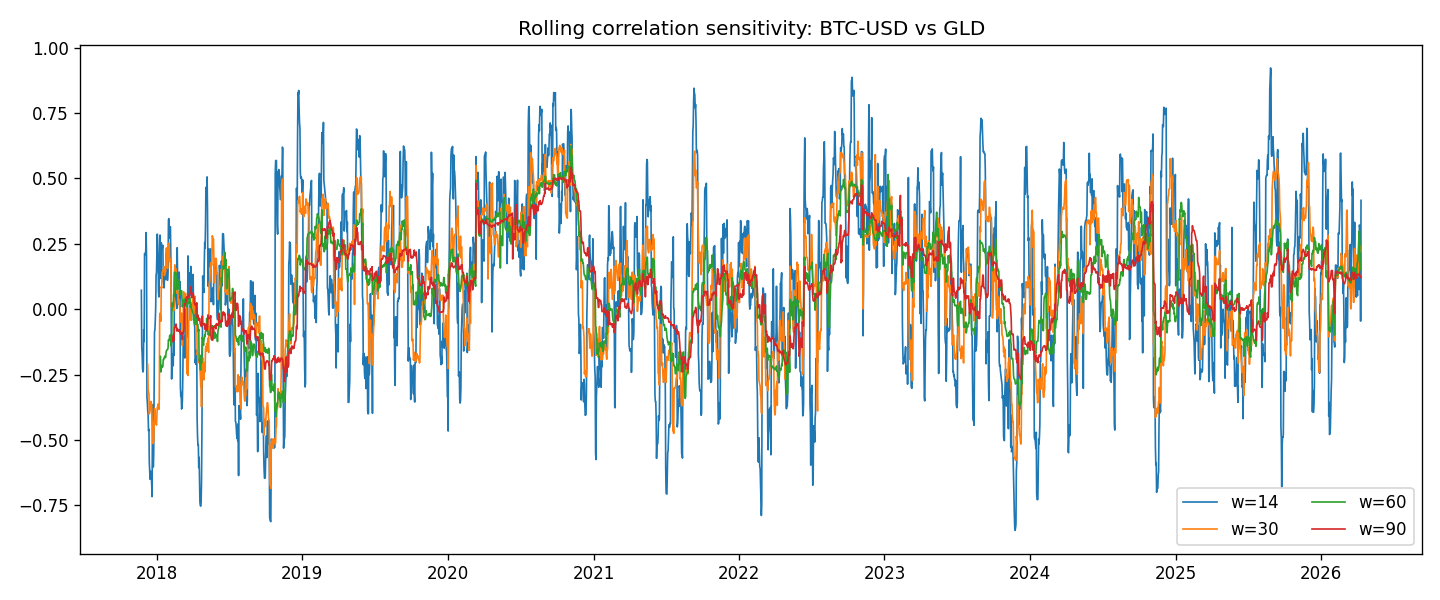
\includegraphics[width=0.9\textwidth]{../outputs/figures/sensitivity_BTC-USD_GLD.png}
    \caption{Sensitivity analysis for the Bitcoin--gold pair.}
    \label{fig:app_sensitivity_gld}
\end{figure}

\begin{figure}[H]
    \centering
    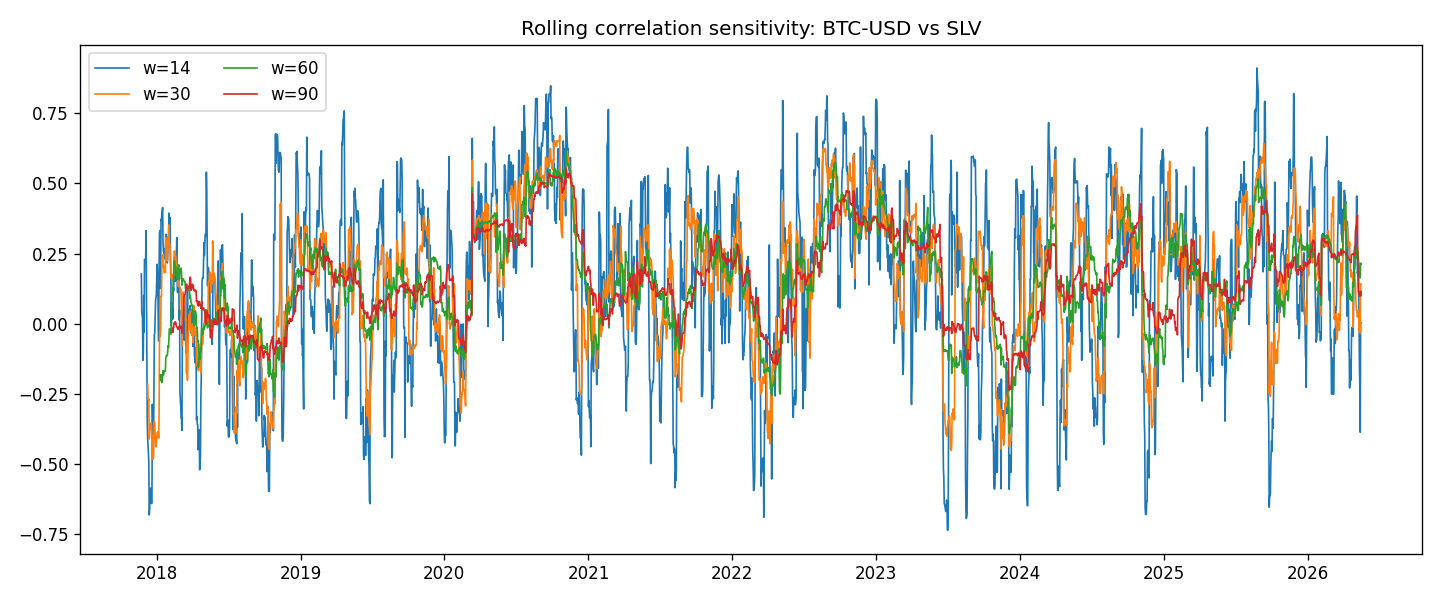
\includegraphics[width=0.9\textwidth]{../outputs/figures/sensitivity_BTC-USD_SLV.png}
    \caption{Sensitivity analysis for the Bitcoin--silver pair.}
    \label{fig:app_sensitivity_slv}
\end{figure}

\begin{figure}[H]
    \centering
    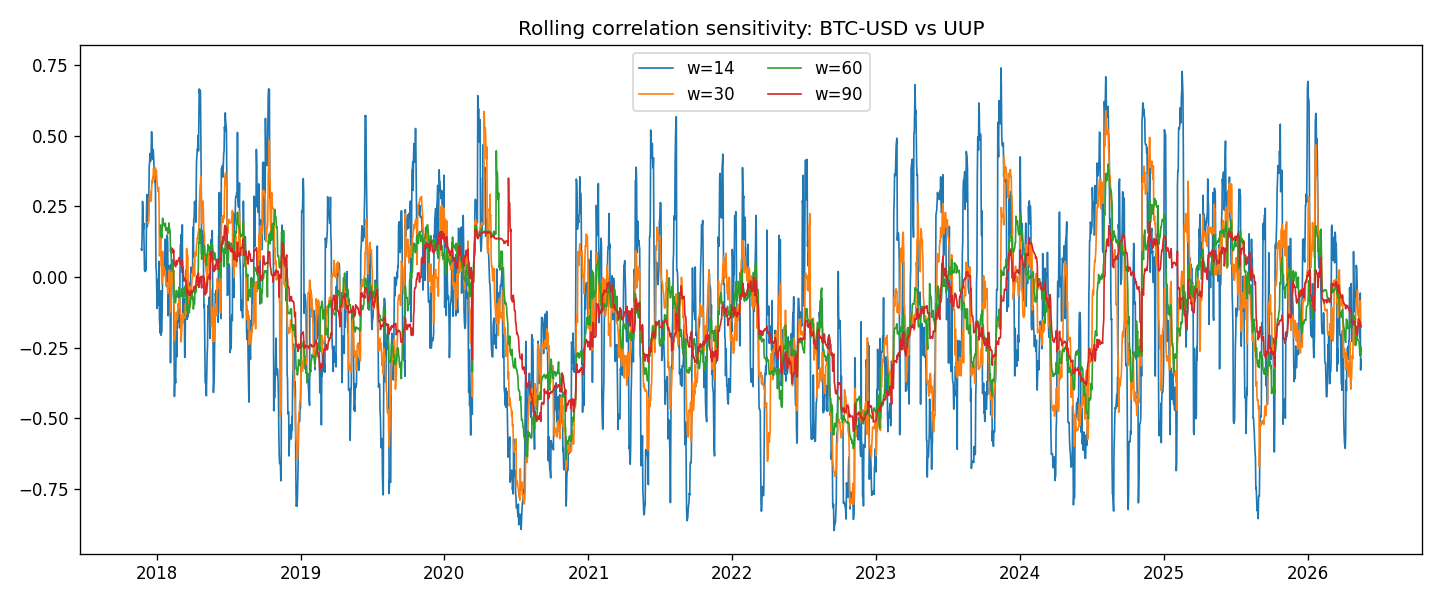
\includegraphics[width=0.9\textwidth]{../outputs/figures/sensitivity_BTC-USD_UUP.png}
    \caption{Sensitivity analysis for the Bitcoin--UUP pair.}
    \label{fig:app_sensitivity_uup}
\end{figure}

\begin{figure}[H]
    \centering
    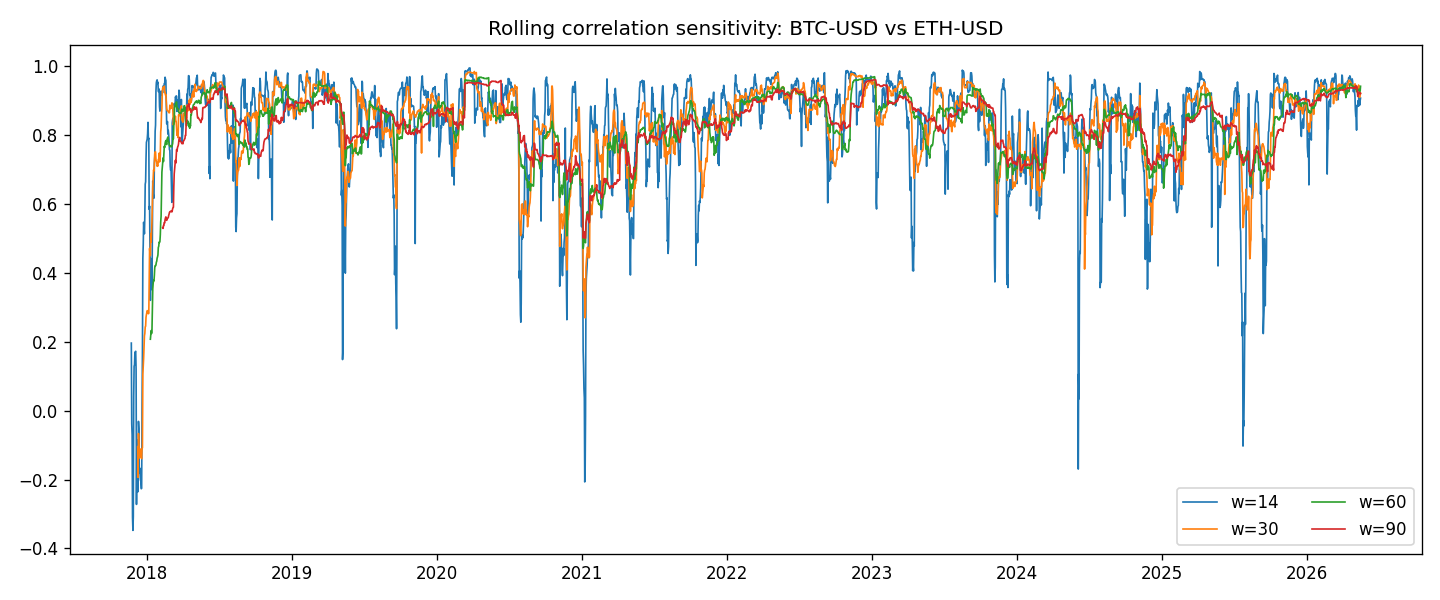
\includegraphics[width=0.9\textwidth]{../outputs/figures/sensitivity_BTC-USD_ETH-USD.png}
    \caption{Sensitivity analysis for the Bitcoin--Ethereum pair.}
    \label{fig:app_sensitivity_eth}
\end{figure}

\needspace{8\baselineskip}
\subsection{Interpretation}

Taken together, these figures reinforce the main text: forecast quality depends heavily on the rolling window, the target stays strongly persistence-driven, and the differences between model families read more clearly off a comparative plot than off any single ranking number.
